The digital control system is designed as a finite state machine with the states illegal, idle, expose and readout as shown in figure~\ref{fig:fsmDiagram}.
The logic connecded to each state is as shown below.

\begin{outline}
  \1 Illegal
  \2 This state is mainly used for resets, it resets all peripherals and set the next state to idle.
  \1 Idle
  \2 This is the normal operating state, the machine allways return to this state eventually.
  \2 In this state exposure increase and exposure decrease are enabled, increase takes presidence over decrease.
  \1 Expose
  \2 The machine normally stays in this state until the exposure time has passed.
  \2 Reset is the only functional input.
  \1 Readout
  \2 The readout sequencer is started, the next state is set to idle afterwards.
  \2 Reset is the only functional input.
\end{outline}


\begin{figure}[htbp]
  \centering
  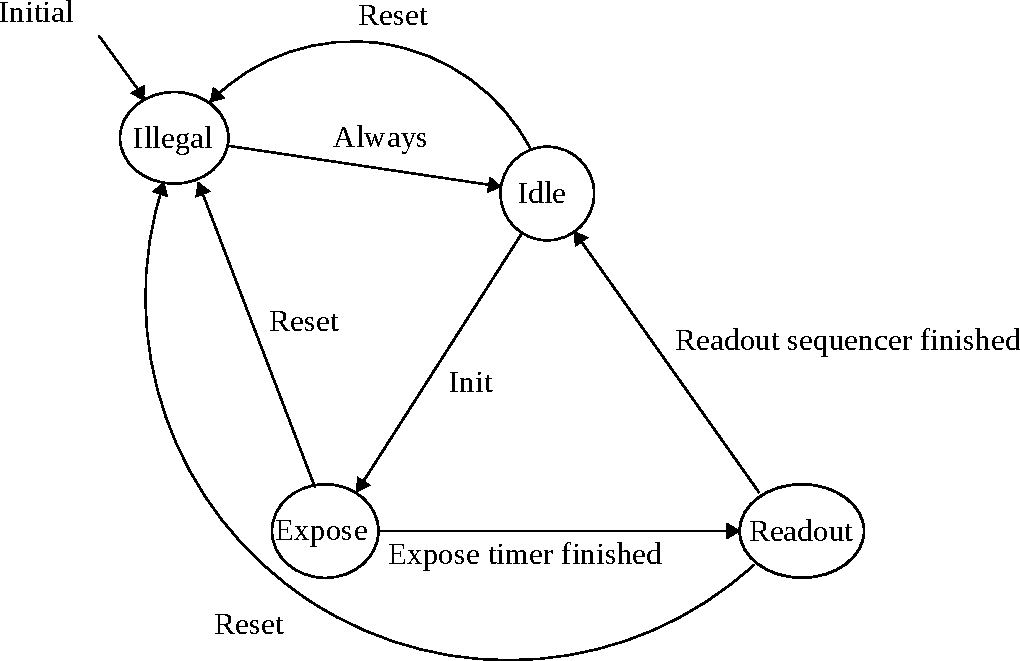
\includegraphics[width=0.85\textwidth]{figures/fsmDiagram}
  \caption{FSM representation of the digital control system}
  \label{fig:fsmDiagram}
\end{figure}
\begin{figure}[htbp]
  \centering
  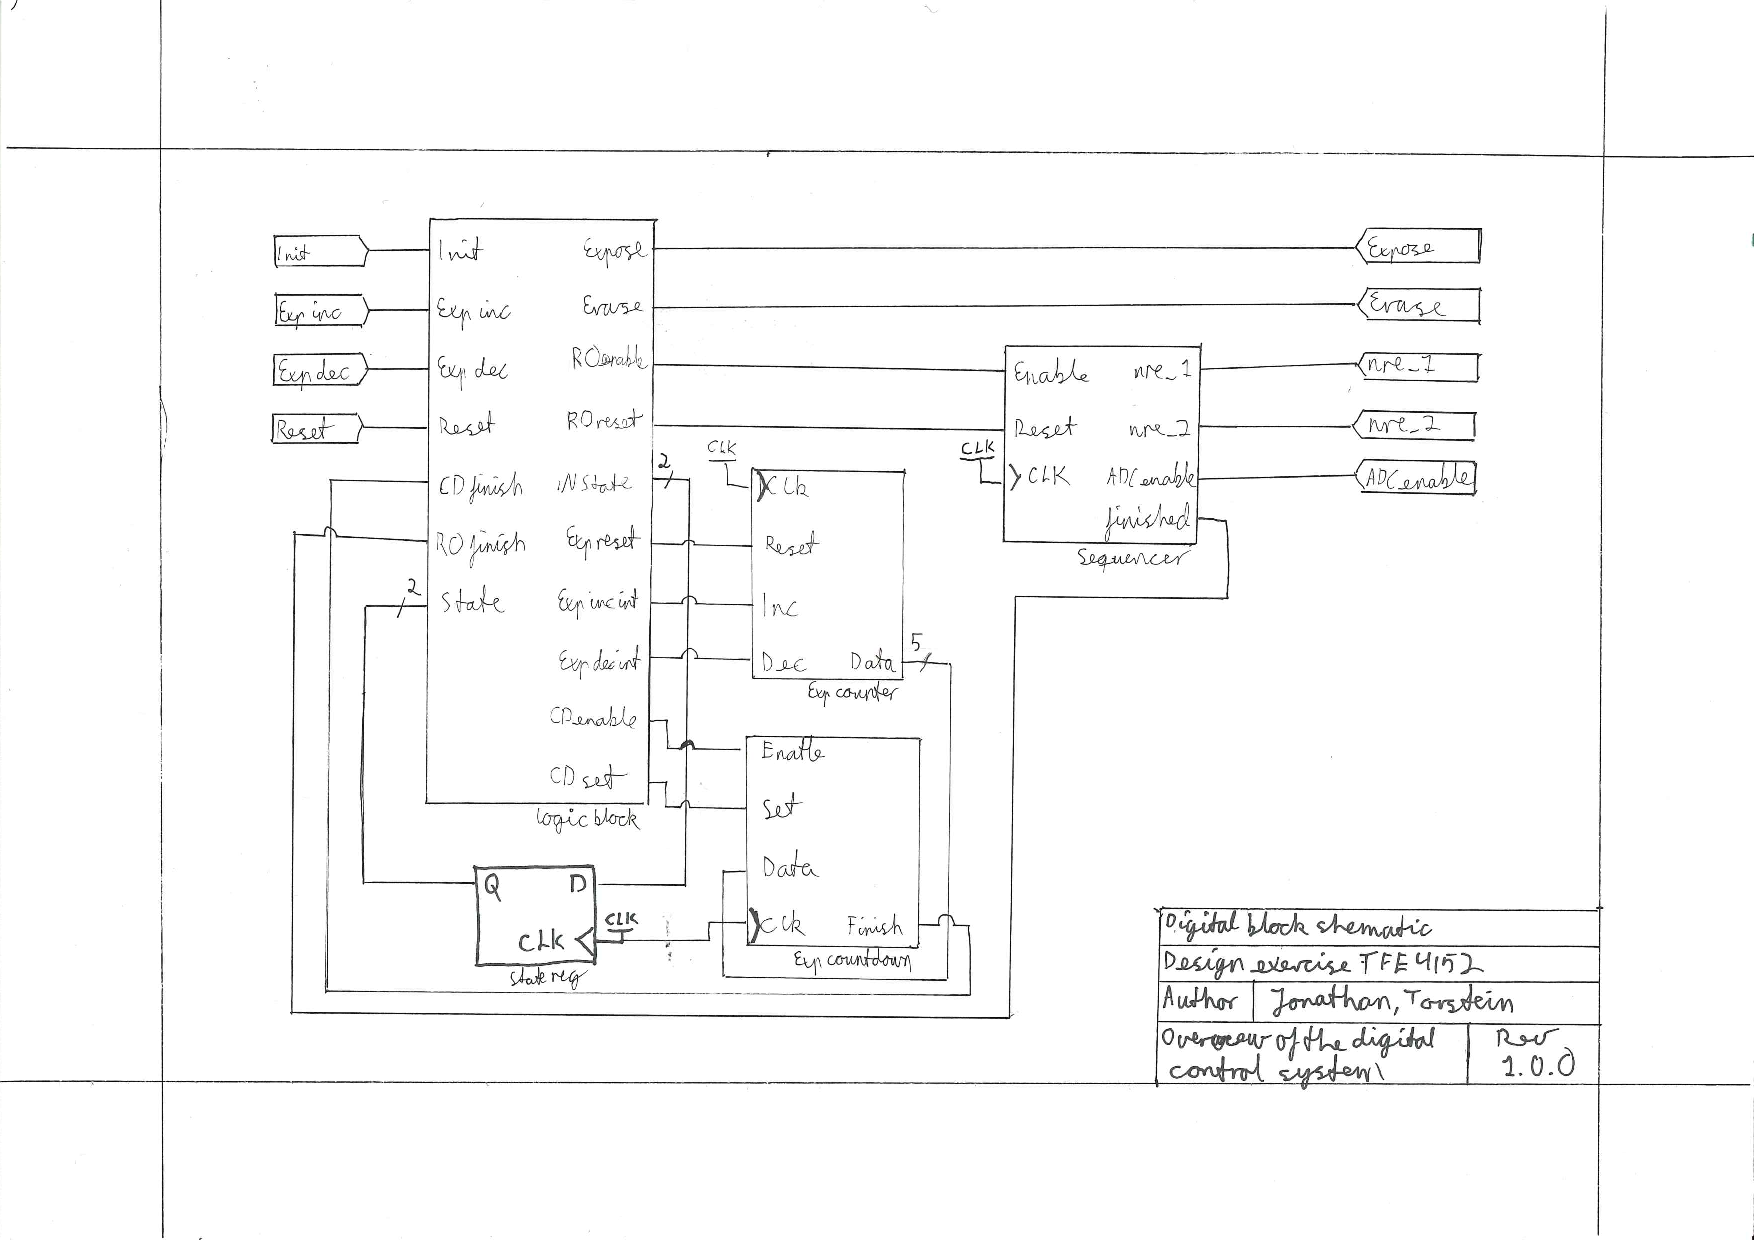
\includegraphics[width=0.85\textwidth]{figures/SchematicDigital}
  \caption{Schematic of the digital design, figure allso found in Appendix~\ref{ap:Schematics}}
  \label{fig:digschematic}
\end{figure}